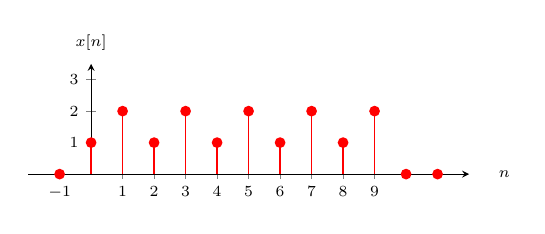
\begin{tikzpicture}[scale=0.8, every node/.append style={font=\scriptsize}]

	\begin{filecontents}{xn.dat}
		n xn
		-1 0
		0 1
		1 2
		2 1
		3 2
		4 1
		5 2
		6 1
		7 2
		8 1
		9 2
		10 0
		11 0		
	\end{filecontents}
	

	

    \begin{axis}[
    		name=axis1,
		y=0.5cm,
		x=0.5cm,
		 clip=false,
		 xmin=-2,xmax=12,
		 xlabel= $n$,
		 ylabel={$x[n]$},
		 ymin=0,ymax=3.5,
		 axis lines=middle,
         	xtick={ -1, 0, 1, 2, 3, 4, 5, 6, 7, 8, 9},
         	%xticklabels={$-\pi$, $\pi$, $2\pi$},
		%ytick={},
		 %yticklabels=\empty,
		 every axis x label/.style={at={(ticklabel* cs:1.05)}, anchor=west,},
		every axis y label/.style={at={(ticklabel* cs:1.05)}, anchor=south,},
     ]
		%\addplot [red, smooth, very thick, mark=none] table [x={omega}, y={X}] {./h_dtft/figures/dtft_square_pulse_N1_2.dat};
		\addplot [red, ycomb,  thick, mark=*] table [x={n}, y={xn}] {./xn.dat};
    \end{axis}


\end{tikzpicture} 